\chapter{Modern Secret Sharing}
Nei precedenti capitoli abbiamo visto come condividere un segreto in modo \textit{sicuro} usando \textbf{Diffie-Hellman} (\cref{def:dh}) oppure \textbf{RSA Key Transport} (\cref{def:rsakey}). In questi casi, la sicurezza proveniva dal fatto che i messaggi scambiati in rete implicavano una difficoltà enorme per un attaccante, che rendeva arduo il tentativo di determinare/rubare la chiave con cui i messaggi vengono cifrati prima di essere scambiati.\\
Vediamo come la crittografia può essere usata non solo per cifrare dei messaggi, ma anche per condividere un segreto.
\begin{example}\label{exam:trivialsecret}
Supponiamo di avere un \textit{Dealer} $D$ e due utenti $A,B$. $D$ genera un segreto di 8 byte (un semplice numero), che spezza in due parti da consegnare agli utenti.\\
Per un segreto di questa dimensione, le probabilità di indovinare il segreto sono chiaramente $1/2^8=1/256$. Supponiamo ora che un \textit{attaccante} $E$ possa intercettare uno dei due messaggi e scoprire metà del segreto. Adesso le probabilità sono $1/2^4=1/16$
\end{example}
\begin{remark}
Dividendo il segreto originale e trasmettendone le due parti, ne riduciamo il livello di sicurezza.
\end{remark}
Il metodo descritto nell'esempio \ref{exam:trivialsecret} è tanto semplice quanto debole, pertanto è lecito chiedersi se sia possibile crearne una versione robustificata.
\section{Trivial Secret Sharing}
\begin{example}
Consideriamo lo scenario dell'esempio \ref{exam:trivialsecret} ma questa volta generiamo una sequenza \textbf{truly random} (una chiave) e facciamone lo xor con il segreto. Otteniamo così un \textbf{Vernam Cipher} (\cref{prop:vernam}). Inviamo adesso ad $A$ la chiave generata randomicamente e a $B$ il risultato dello xor. Osserviamo che:\\
\begin{itemize}
    \item Se $E$ riuscisse ad intercettare il messaggio di $A$, non avrebbe alcun vantaggio in quanto il numero casuale da lui generato non contiene informazioni sul segreto originale.
    \item Se $E$ riuscisse ad intercettare il messaggio di $B$, il quale contiene la chiave, non avrebbe alcun vantaggio in quanto l'operazione di xor effettuata con una quantità \textbf{truly random} genera un risultato altrettanto randomico, la cui probabilità di essere indovinato dopo aver ricevuto un messaggio non si abbassa e resta $1/2^8=1/256$.
\end{itemize}
\end{example}
\begin{figure}[ht]
    \centering
    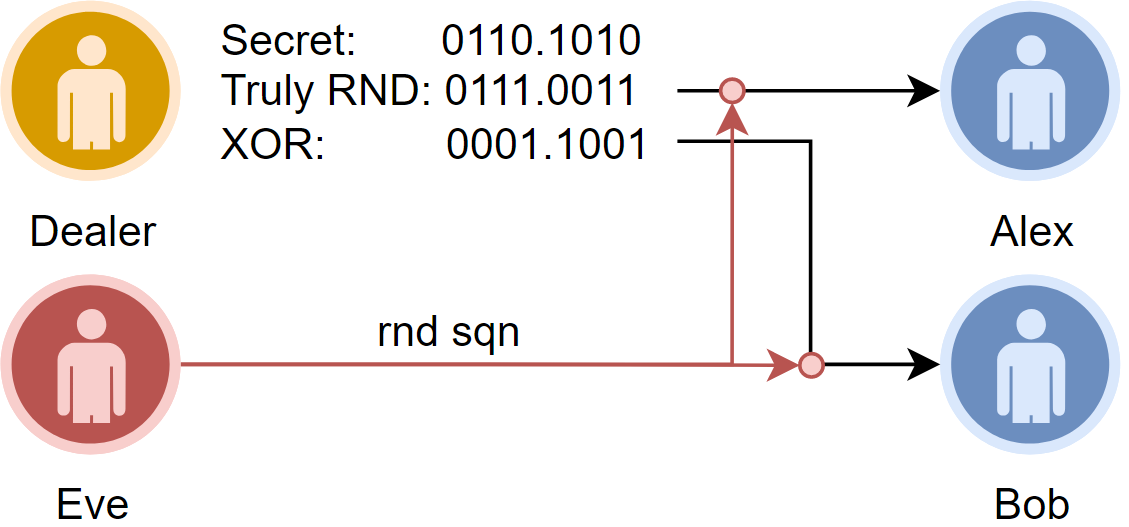
\includegraphics[width=0.6\textwidth]{image/secret_sharing/trivialsecret.png}
    \caption{Trivial Secret Sharing}
    \label{fig:trivialsecret}
\end{figure}
Distinguiamo tra il segreto originale e le parti in cui viene suddiviso e consideriamo il teorema:
\begin{definition}[Shares]\label{def:shares}
Uno Share è una delle parti in cui viene suddiviso un secreto.
\end{definition}\pagebreak
\begin{theorem}[Modular Sum as XOR equivalent]
L'operazione di XOR-ing non è necessaria. Si può dimostrare che al posto dello xor è possibile effettuare una \textbf{somma modulare}, poiché se uno degli addendi è truly random, il risultato sarà nuovamente truly random.
\end{theorem}
\begin{example}
Consideriamo un secret $S=0010.1101\rightarrow 45$ e un $RAND\mod256=180$. $S-RAND\mod{256}=-135\mod{256}=121$. $A$ riceverà 180, $B$ 121. Il segreto che le parti potrenno ricomporre sarà quindi dato da: $180+121\mod{256}=45$.
\end{example}
\begin{note}
Questo fatto è interessante poiché stiamo usando l'algebra già contenuta nei calcolatori moderni (a seconda della parola usata stiamo facendo somme in modulo 32, 64bit ecc.) ed è più facile da implementare rispetto ad una algebra bitwise.
\end{note}
Supponiamo ora di dover dividere il segreto in $n$ parti. Possiamo condividere il segreto nella seguente modalità.
\begin{theorem}[Trivial Secret Sharing]\label{thm:trivialsecret}
Generiamo un segreto $S$ all'interno di un range $K$. Per condividerlo con $n$ parti dobbiamo:
\begin{enumerate}
    \item Generare $n-1$ quantità $r\mod{K}$ \textbf{truly random}.
    \item Inviare alle $n-1$ parti uno degli shares generati precedentemente.
    \item Inviare all'$n$-esima parte $S-\sum_{i=1}^{n-1}{r_i}$,
\end{enumerate}
Finché $n-1$ shares vengono rilevati, un avversario ha \textbf{ancora} probabilità di indovinare il segreto pari a $1/\text{\#bit}(S)$. Per indovinare il segreto sono necessarie \textbf{tutte le $n$} parti.
\end{theorem}
\section{Shamir Secret Sharing}
La versione moderna e più utilizzata per condividere un segreto è attribuita a Shamir. Per affrontare questo schema di condivisione, definiamo:
\begin{definition}[N out of N Secret Sharing]\label{def:noutn}
Uno schema di condivisione \textbf{(n,n)} "N out of N" condivide il segreto con $n$ persone e necessita che \textbf{tutte} ed $n$ siano "presenti" per rivelarlo.
\end{definition}
\begin{definition}[T out of N Secret Sharing]\label{def:toutn}
Uno schema di condivisione \textbf{(t,n)} "T out of N" condivide il segreto con $n$ persone e necessita che \textbf{solo} $t$ siano "presenti" per rivelarlo.\\
\begin{remark}
$1<t<n$. Se $t=1$, ogni parte conosce il segreto.
\end{remark}
\end{definition}
\begin{note}
Un esempio di schema (n,n) è il trivial secret sharing \cref{thm:trivialsecret}
\end{note}
Il secondo schema è molto più robusto poiché permette di ricostruire un segreto anche se non tutte le parti che lo conoscono sono presenti. L'idea alla base dello schema proposto da Shamir è la seguente:
\begin{wrapfigure}{r}{0.4\textwidth}
  \vspace{-20pt}
  \begin{center}
    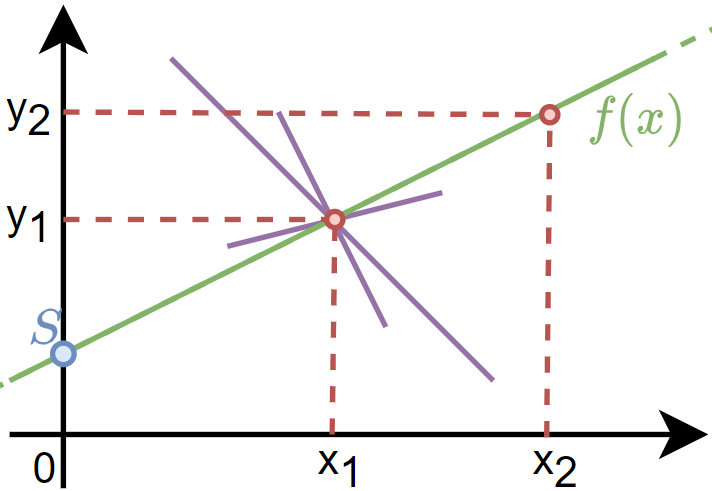
\includegraphics[width=0.4\textwidth]{image/secret_sharing/rectfind.png}
  \end{center}
  \vspace{-20pt}
  \caption{2 point to find a rect}
  \label{fig:rectfind}
  \vspace{-10pt}
\end{wrapfigure}
\begin{example}[ (2,n) Secret Sharing]\\
Consideriamo una retta in un piano cartesiano. \\Quanti punti sono necessari per identificare univocamente tale retta?
\begin{note}
Sappiamo che servono \textbf{2 punti} per identificare univocamente la retta e che per un punto ne passano infinite.
\end{note}
Sia $f(x)$ la retta in questione. Se poniamo il \textbf{segreto} come \textbf{$S=f(0)$}, possiamo assegnare i diversi \textbf{shares} come p\textbf{unti qualsiasi sulla retta}. Unendo due punti, la retta è univocamente determinata e calcolandone il valore nell'origine possiamo trovare il segreto. Se invece abbiamo solo uno shares, è impossibile determinare il segreto poiché esistono infinite rette che passano per quel punto.
\end{example}
Possiamo riassumere l'idea di base con il seguente teorema:
\begin{theorem}[(2,n) Rect Secret Sharing]\label{thm:rectsecret}
\begin{enumerate}
\item Generare un coefficiente $a$ truly random e un segreto $S$. La retta risultante sarà: \[y=S+a\cdot x\]
    \item Numerare i partecipanti in modo ordinato da $1$ a $n$.
    \item Scegliere a priori, in modo randomico ed esclusivo, le $x_i$ da assegnare.
    \item Comunicare ai partecipanti il loro numero e la corrispondente $x_i$.
\end{enumerate}
Per ogni partecipante, avremo un punto $p_i=(x_i,y_i)$.\footnotemark\\
\footnotetext{\textsuperscript{\thefootnote}Poiché il numero assegnato a ogni partecipante è noto a priori, è possibile salvare esclusivamente il valore $y_i$ per semplicità, piuttosto che l'intero punto come share.}
Per ricostruire il segreto possiamo procedere per interpolazione:
\begin{enumerate}
    \item Dati $p_i=(x_i,y_i)$ e $p_j=(x_j,y_j)$, allora:
    \[\frac{y-y_i}{y_j-y_i}=\frac{x-x_i}{x_j-x_i}\Longrightarrow y=y_i+\frac{x-x_i}{x_j-x_i}(y_j-y_i)\]
    \item Porre $x=0$ e trovare $y=S$:\footnotemark
    \[S=y_j\frac{-x_i}{x_j-x_i}+y_i\frac{-x_j}{x_j-x_i}\]
\end{enumerate}
\footnotetext{\textsuperscript{\thefootnote}Il segreto non verrà mai usato da nessuno dei partecipanti in quanto il valore $x=0$ è precluso agli altri.}
\end{theorem}\pagebreak
E generalizzarla rispetto ad un polinomio di grado $t-1$.


\begin{corollary}[Lagrange Interpolation]\begin{wrapfigure}{r}{0.4\textwidth}
  \vspace{-20pt}
  \begin{center}
    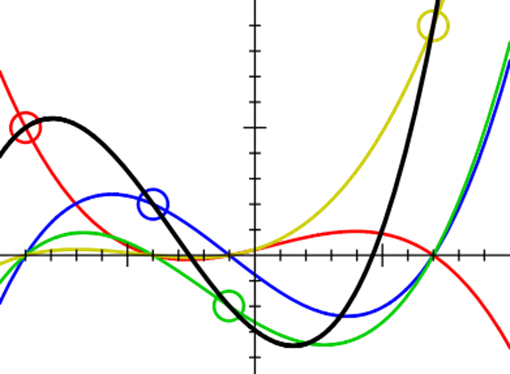
\includegraphics[width=0.3\textwidth]{image/secret_sharing/poly.png}
  \end{center}
  \vspace{-20pt}
  \caption{Polynomials interpolation}
    \label{fig:polyinter}
  \vspace{-10pt}
\end{wrapfigure}
Un qualsiasi polinomio di grado $t-1$, con $t$ punti \textbf{noti} $(x_1,y_1),\dots,(x_{t-1},y_{t-1})$, è sempre decomponibile nella forma:
\begin{equation}\label{eq:lagrangeinter}
    y=\sum_{i=1}^{t}y_i\Lambda_i(x)
\end{equation}
Dove $\Lambda_i(x)$ è la \textbf{base/polinomio di Lagrange} definita come:
\begin{equation}
    \begin{gathered}\label{eq:lagrangebase}
    \Lambda_i(x)  = \prod_{m=1,m\ne i}^{t}\frac{x-x_m}{x_i-x_m}=\frac{x-x_1}{x_i-x_1}\dots\frac{x-x_{i-1}}{x_i-x_{i-1}}\frac{x-x_{i+1}}{x_i-x_{i+1}}\dots\frac{x-x_t}{x_i-x_t}\\
    \Lambda_i(x_i) = 1,\,\,\Lambda_i(x_m)=0\,\,\text{for}\,m\ne i
\end{gathered}
\end{equation}
\end{corollary}
\begin{remark}
In parole povere, una base di lagrange è un polinomio definito come 1 quando calcolato nello share da cui deriva, e 0 per gli altri shares. Questo perché quando calcoliamo una base in un altro shares un numeratore sarà sicuramente nullo ed annullerà tutto il prodotto, quando calcolata nel suo shares, invece, tutti i termini si semplificheranno.
\end{remark}
\begin{theorem}[(t,n) Shamir's Secret Sharing Scheme]\label{thm:tnsecret}
Come Dealer:
\begin{enumerate}
    \item Genera un polinomio $p(x)$ di grado $t-1$ con \textbf{coefficienti truly random} $a_i$.
    \item Seleziona un segreto $S$ come termine noto del polinomio.
    \item Distribuisci uno share ad ognuno degli $n$ partecipanti, come: 
    $(x_i,y_y)$ con $ y_i=p(x_i)$
\end{enumerate}
Per \textbf{ricostruire il segreto}:
\begin{enumerate}
    \item Raccogli \textbf{t} degli \textbf{n} shares disponibili.
    \item Calcola il segreto usando L'interpolazione di lagrange (\cref{eq:lagrangeinter}) con $x=0$
    \begin{equation}\label{eq:tnsecret}
        S=\sum_{\text{shares }x_i}y_i\Lambda_{x_i}\,\,\,\text{con}\,\,\Lambda_{x_i}=\Lambda_{x_i}(0)=\prod_{\text{shares }x_k\ne x_i}\frac{-x_k}{x_i-x_k}
    \end{equation}
\end{enumerate}
\end{theorem}
\begin{note}
Il polinomio di lagrange può essere \textbf{precalcolato} in quanto non contiene alcun valore che non sia lo share i-esimo o gli altri k selezionati per ricostruire il segreto.
\end{note}\pagebreak
\begin{example}
\label{exam:shamirex}
Consideriamo uno scenario (3,n). Il dealer deve generare un polinomio di grado $t-1=3-1=2$, ovvero una parabola. Supponiamo: \[y=32+52x+3x^2\]
Supponiamo di avere 4 partecipanti, pertanto avremo bisogno di generare e distribuire 4 shares fatti da $(x_i, y_i)$, ma soltanto 3 saranno necessari a ricostruire il segreto. Supponiamo di usare $1,2,3$.
\begin{multicols}{2}
    \begin{itemize}
    \item $x=1\rightarrow$ share: $(1,87)$
    \item $x=2\rightarrow$ share: $(2,148)$
    \item $x=3\rightarrow$ share: $(3,215)$
    \item $x=4\rightarrow$ share: $(4,288)$
\end{itemize}
\columnbreak
\begin{equation*}
\begin{aligned}
\Lambda_1&=\frac{-x_2}{x_1-x_2}\cdot\frac{-x_3}{x_1-x_3}&=\frac{-2}{1-2}\cdot\frac{-3}{1-3}&=3\\
\Lambda_2&=\frac{-x_1}{x_2-x_1}\cdot\frac{-x_3}{x_2-x_3}&=\frac{-1}{2-1}\cdot\frac{-3}{2-3}&=-3\\
\Lambda_3&=\frac{-x_1}{x_3-x_1}\cdot\frac{-x_2}{x_3-x_1}&=\frac{-1}{3-1}\cdot\frac{-2}{3-2}&=1
\end{aligned}    
\end{equation*}
\end{multicols}
Ricostruiamo il segreto con: $s=y_1\Lambda_1+y_2\Lambda_2+y_3\Lambda_3=87\cdot3+148\cdot(-3)+215\cdot1=32$
\begin{remark}
Il modello usato in questo esempio è sicuro, in quanto per ricalcolare il segreto \textbf{SERVE} che 3 shares vengano messi "insieme".
\end{remark}
\begin{remark}
Se avessimo calcolato il prodotto $\sum_{i=1}^3y_i\Lambda_i$ \textbf{senza sostituire $x=0$} avremmo ritrovato il polinomio di partenza.
\end{remark}
\end{example}
\begin{proposition}[Perfect Security of Shamir's Scheme]\label{prop:shamirsecurity}
Lo schema di Shamir è sicuro a patto che i calcoli vengano fatti in aritmetica modulare. In particolare, \textbf{sia} il \textbf{segreto} che i \textbf{coefficienti del polinomio} \textbf{devono} essere presi nel \textbf{campo dei numeri primi}.\footnotemark
\footnotetext{\textsuperscript{\thefootnote}Il numero primo scelto non deve essere \textbf{necessariamente grande}, ma sufficientemente grande per garantire di avere un segreto all'interno dell'intervallo scelto. Ad esempio, per $s\in(1,100)$ $p=101$ è un buon numero primo.}
\end{proposition}
Infatti, prendendo una parabola, abbiamo soltanto un sottoinsieme di valori che possiamo utilizzare e questo restringe il campo di probabilità rispetto ad un brute-force. Rispetto all'esempio \ref{exam:shamirex} supponiamo:
\begin{itemize}
    \item $S\in [1,100]$ distribuito in modo uniforme.
    \item Di \textbf{conoscere} il \textbf{primo} e il \textbf{terzo} share.
\end{itemize}
Per calcolare il secondo share, si può procedere per brute-force calcolando:
\[
s=y_1\Lambda_1+y_2D+y_3\Lambda_3=87\cdot3+D\cdot(-3)+215\cdot1=476-3D
\]
Per ogni valore \textbf{intero} $D$. In particolare, si può vedere come per $D\in(125,158)$ il valore di $S$ assume valori nell'intervallo $[2,98]$ con un passo di $3$ per ogni tentativo effettuato. Questo significa che sull'intervallo aperto $(1,100)$ con probabilità $p=1/3$ il segreto può essere rivelato.
\begin{note}
La conoscenza di due shares su tre \textbf{aumenta} la \textbf{probabilità} di \textbf{indovinare il segreto}, fornendo informazioni all'attaccante.
\end{note}
Questo esempio ci permette di definire il concetto di sicurezza in due modi diversi:
\begin{definition}[Computational Security]
Uno schema \textbf{computational Secure} non fornisce all'attaccante un modo \textbf{efficiente}\footnotemark per calcolare il segreto.
\footnotetext{\textsuperscript{\thefootnote}Vedi \textbf{Discrete Logarithm Problem} o \textbf{Fattorizzazione RSA} (\cref{prop:disclog,prop:prodfact}).}
\end{definition}
\begin{definition}[Unconditionally Security]
Uno schema \textbf{Unconditionally Secure} non fornisce all'attaccante alcuna possibilità di calcolare un segreto se \textbf{uno o più} dati sono mancanti.
\end{definition}
Lo schema di Shamir è \textbf{Unconditionally Secure}, perché matematicamente se uno share è mancante anche se un'attaccante ha sufficiente potenza di calcolo non potrebbe mai ricostruire il segreto. Vediamo ora cosa succede usando aritmetica modulare con numeri primi.
\begin{example}\label{exam:shamirmodular}
Consideriamo uno scenario (3,n). Il dealer deve generare un polinomio di grado $t-1=3-1=2$, ovvero una parabola. Supponiamo: \[y=3 x^2+52 x+32
   \bmod 101\]
Dove il segreto $s=32\in(1,100)$ e il numero primo scelto è $p=101$. Con 4 partecipanti avremo bisogno di generare e distribuire 4 shares ma supponiamo di usare $1,2,4$ per ricostruire il segreto. Per provare che è possibile non seguire l'ordine cardinale nell'assegnazione degli share, assegniamo $x_4=6$.\\
Facendo i calcoli abbiamo:
\begin{equation*}
    \begin{aligned}
    y_1&=y(x_1)&=87,    &&  \Lambda_1&=(-x_2)(-x_4)\bmod101\cdot[(x_1-x_2)(x_1-x_4)]^{-1}\bmod101=63\\
    y_2&=y(x_2)&=47,    &&  \Lambda_2&=(-x_1)(-x_4)\bmod101\cdot[(x_2-x_1)(x_2-x_4)]^{-1}\bmod101=49\\
    y_3&=y(x_3)&=13,    &&  &\text{Non va calcolato.}\\
    y_4&=y(x_4)&=48,    &&  \Lambda_4&=(-x_1)(-x_2)\bmod101\cdot[(x_4-x_1)(x_4-x_2)]^{-1}\bmod101=91
    \end{aligned}
\end{equation*}
\begin{note}
Ovviamente con aritmetica modulare non possiamo usare le divisioni, ma dobbiamo moltiplicare per l'inversa modulare.
\end{note}
A questo punto possiamo ricostruire il segreto semplicemente moltiplicando i tre fattori:
\[
s=[y_1\Lambda_1+y_2\Lambda_2+y_3\Lambda_3]\bmod101=[87\cdot63+47\cdot49+48\cdot91]\bmod101=32
\]
\begin{remark}
Supponiamo ora di attaccare lo schema, conoscendo il secondo e il quarto share e il range di valori in cui il segreto può essere contenuto. Dovremmo risolvere l'equazione:
\[s=[\Lambda_1\cdot D+Lambda_2+y_3\Lambda_3]\bmod101=[5+63D]\bmod101\]
Se adesso proviamo un qualsiasi valore di $D$ nell'intervallo in cui il segreto può esistere vedremmo che i risultati ottenuti sarebbero \textbf{tutti i numeri da 1 a 100} in modo \textbf{uniformemente distribuito}. Questa proprietà è dovuta ovviamente all'operazione di modulo e garantisce unconditional security anche se sono noti due share su tre. 
\end{remark}
\end{example}\pagebreak
\begin{note}
Quando utilizziamo schemi Computational Secure in realtà stiamo facendo \textbf{Computation Hiding}. Ovvero, nascondiamo un segreto tramite una funzione Hash (anche la più resistente al mondo), che dipende sempre e comunque dallo spazio dei valori assunti dal segreto. Più questo sarà grande, più sarà difficile per un attaccante riuscire ad indovinare il segreto tramite \textbf{enumeration attack}.
\end{note}
\begin{corollary}[Ideality of Secret Sharing Scheme]
Uno schema di condivisione di segreti è \textbf{ideale} se \textbf{tutti} gli \textbf{share} hanno \textbf{dimensione} \textbf{almeno pari} a quella del segreto. Se gli share fossero più piccoli, una volta che almeno uno è noto sarebbe più facile ricostruire il segreto a causa dell'entropia ridotta.
\end{corollary}
\begin{note}
Lo schema di Shamir è ideale.\textbf{ Lo schema proposto da Blakley era invece basato su share di dimensione t-volte quella del segreto.}
\end{note}
\subsection{Secret Sharing for Multipart Computation}
Introduciamo una proprietà di cui gode lo schema di Shamir:
\begin{proposition}[Homomorphic Property of Shares]\label{prop:homomorphic}
Poiché gli share in uno schema di Shamir sono generati a partire da polinomi, allora vale che: \textbf{la somma degli shares è uguale allo share della somma dei segreti}. Ovvero:
\begin{equation}\label{eq:homomorphic}
    f_i+g_i = (f+g)_i
\end{equation}
Dove $f_i,g_i$ sono due polinomi che definiscono un segreto e gli share sono $\{k_i,y_i(k_i)\}$
\end{proposition}
Questa proprietà permette di usare lo schema anche nel caso in cui invece di essere interessati alla ricostruzione di un segreto in particolare, siamo interessati alla ricostruzione della somma di più segreti.\\
Tipicamente l'approccio normale sarebbe il seguente:
\begin{enumerate}
    \item Ricostruisco il segreto $S_1$.
    \item Ricostruisco il segreto $S_2$.
    \item Calcolo $S_1+S_2$.
\end{enumerate}
Per la \cref{prop:homomorphic} invece possiamo procedere come segue:
\begin{enumerate}
    \item sia $\alpha_1$ il segreto dato da $f_i(k)+g_i(k)$.
    \item sia $\alpha_2$ il segreto dato da $f_i(v)+g_i(v)$.
    \item Usando \cref{eq:homomorphic} possiamo ricostruire la somma $\alpha_1+\alpha_2$ \textbf{SENZA CONOSCERE} né il segreto $\alpha_1$ né $\alpha_2$.
\end{enumerate}
Questa modalità di calcolare un segreto è detta: \textbf{Secure Multiparty Computation} e costituisce una branca della crittografia utile ad esempio in scenari finanziari (Si vuole sapere chi ha fatto una donazione ma non quanto), medici, controllo del traffico ecc. \pagebreak
\begin{definition}[Secure Multiparty Computation]\label{def:smc}
Calcolo del risultato di una funziona senza rilevare i dati in input. Formalmente: 
\begin{itemize}
    \item Per $N$ partecipanti $P_1,...,P_n$ associa un valore $z_i$.
    \item Calcola la funzione $f(z_1,z_2,...,z_n)$ tale che il \textbf{risultato} sia \textbf{pubblico} ma \textbf{nessuna informazione} su un qualsiasi $z_i$ è deducibile dal risultato di $f$.
\end{itemize}
\begin{remark}
Si può dimostrare che è possibile \textbf{effettuare} \textbf{qualsiasi calcolo} a patto di avere sufficiente potenza di calcolo.
\end{remark}
\end{definition}
Lo SMC è una tecnica che torna comoda quando utilizziamo una \textbf{somma pesata}, che può essere calcolata in modo \textbf{molto efficiente}. In particolare, per caso in cui vogliamo garantire una certa confidenzialità come ad esempio scenari di calcolo salariale medio di una popolazione o consumo energetico, possiamo suddividere un'unica grande trusted third party in diversi enti che possono garantire per la privacy dell'utenza che non comunicando tra loro (a meno di collusioni eventuali) possono oscurare il dato privato del singolo utente.
\begin{figure}[h]
    \centering
    \begin{subfigure}[b]{0.4\textwidth}
    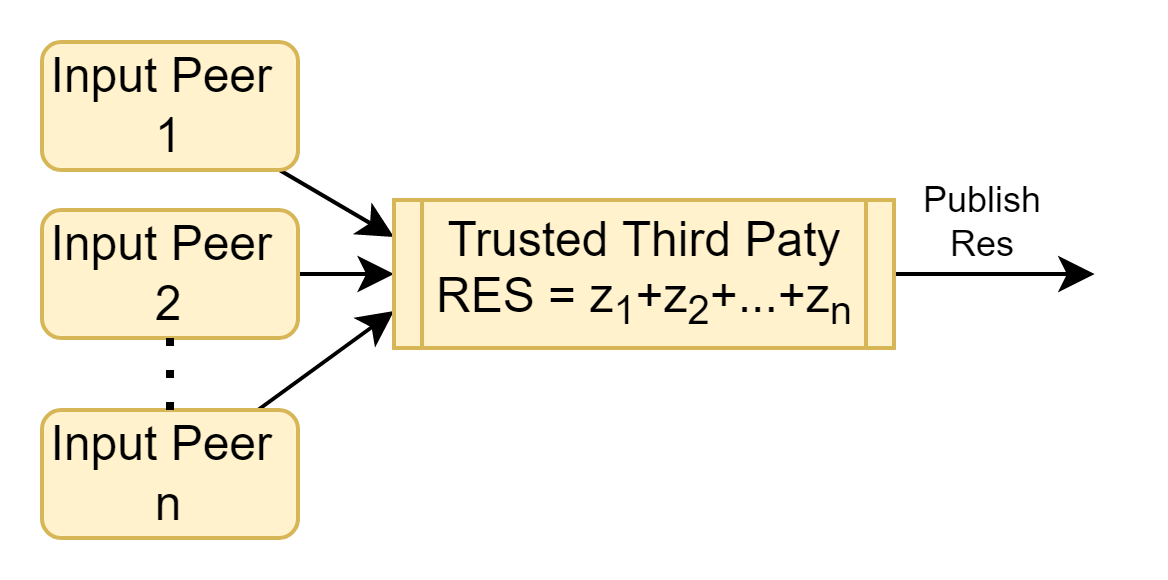
\includegraphics[width=\textwidth]{image/secret_sharing/ttp.png}
    \caption{Trusted Third Party w/o SMC}
    \label{fig:ttp}
    \end{subfigure}\quad
    \begin{subfigure}[b]{0.5\textwidth}
    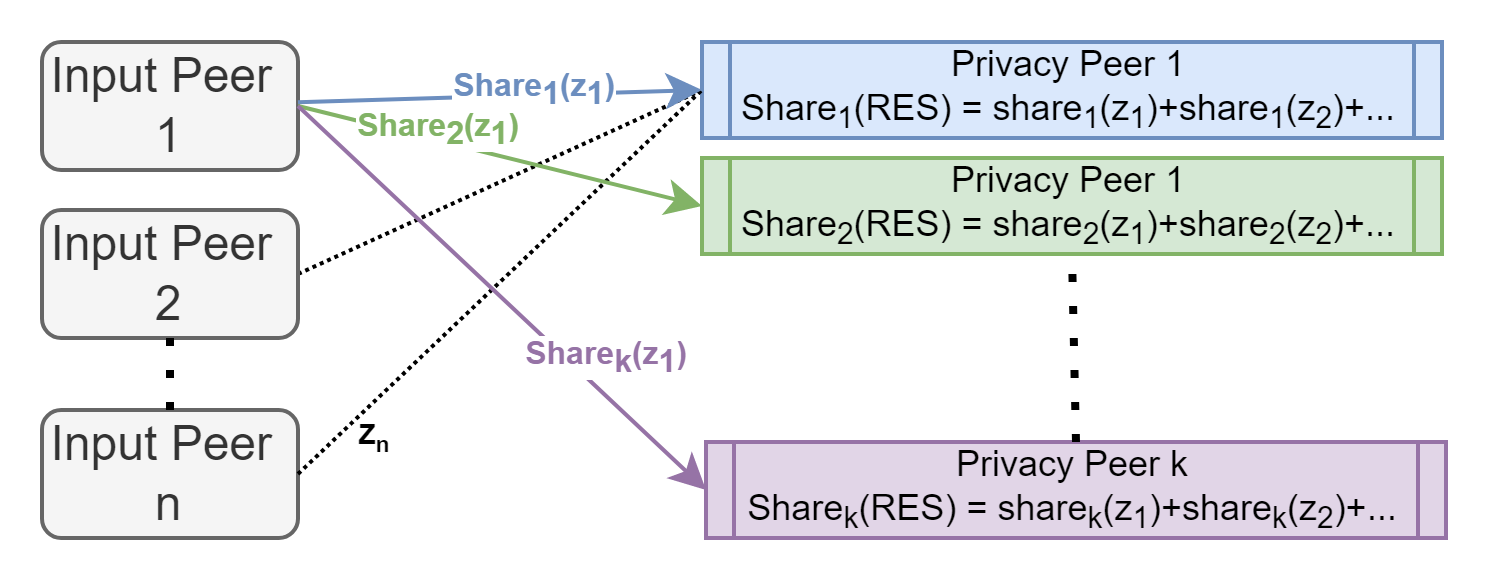
\includegraphics[width=\textwidth]{image/secret_sharing/simulatedttp.png}
    \caption{Simulated TTP w/ SMC}
    \label{fig:smcttp}
    \end{subfigure}
    \caption{SMC example}
\end{figure}\\
Il vantaggio fondamentale è il deployment del sistema:
\begin{corollary}[SMC Deployment]
\begin{itemize}
    \item Possiamo avere da $3$\footnotemark a $n$ input peer e migliaia di end-user.
    \item Possiamo avere da $2$ a $k$ privacy peer, e l'aumentare di questo numero aumenta il livello di sicurezza del sistema.
    \item Possiamo usare uno schema di Shamir, per usare un numero qualsiasi di privacy peer, pagando il prezzo di aritmetica modulare con numeri primi.
\end{itemize}
\footnotetext{\textsuperscript{\thefootnote}Se avessimo 2 input una delle parti potrebbe dedurre il valore privato per sottrazione.}
\end{corollary}\pagebreak
\begin{theorem}[SMC with Shamir Scheme]
Come Input Peer $i$-esimo.\footnotemark
\begin{itemize}
    \item Per $N$ partecipanti $P_1,...,P_n$ associa un valore $z_i$.
    \item Genera polinomi $p_i(x)$ di grado $t-1$.
    \item Invia privatamente gli shares $p_i(1),...,p_i(k)$ ai privacy peer $1,...,k$.
\end{itemize}
\footnotetext{\textsuperscript{\thefootnote}Non serve ci sia coordinazione tra gli input peer.}
Come Privacy Peer $m$-esimo:
\begin{itemize}
    \item Raccogli gli shares in input $p_1(m),p_2(m),...,p_k(m)$.
    \item Calcola $RES(m)=p_1(m)+p_2(m)+...+p_k(m)$.
    \item Pubblica il risultato aggregato $RES(m)$.
\end{itemize}
Come End-User, possiamo ricostruire il risultato tramite lagrange interpolation.
\end{theorem}
\begin{example}[ Input Peers as Privacy Peers]\\
Un esempio pratico è quello nel quale vi è la necessità in un gruppo di utenti di scambiarsi dati in forma anonima, come ad esempio una votazione in una cerchia ristretta. Lo schema da adottare è (n,n) poiché tutti devono partecipare. In questo caso gli input peers possono agire come privacy peers a rotazione, senza che nessuno riveli mai il proprio segreto.\\
In particolare, possiamo procedere nel seguente modo:
\begin{itemize}
    \item L'entità \textit{i-esima} \textbf{fa da dealer} e genera $n-1$ share $R_i$ randomicamente e \textbf{trattiene per se} lo share $R_1$.
    \item La stessa entità invia gli share alle altre entità, inviando all'ultima la quantità: \[(S_i-\sum_{i=1}^{n-1}R_i)\bmod N\]
    \item \textbf{A rotazione}, tutti i partecipanti fanno da dealer, tranne l'ultimo.
    \item L'entità \textit{n-esima} invia alle altre entità i suoi share e trattiene per se la quantità \[(S_i-\sum_{i=1}^{n-1}R_i)\bmod N\]
\end{itemize}
Vediamo un esempio con schema (3,3) in \cref{fig:inputprivacy}
\begin{figure}[h]
\vspace{-10pt}
    \centering
    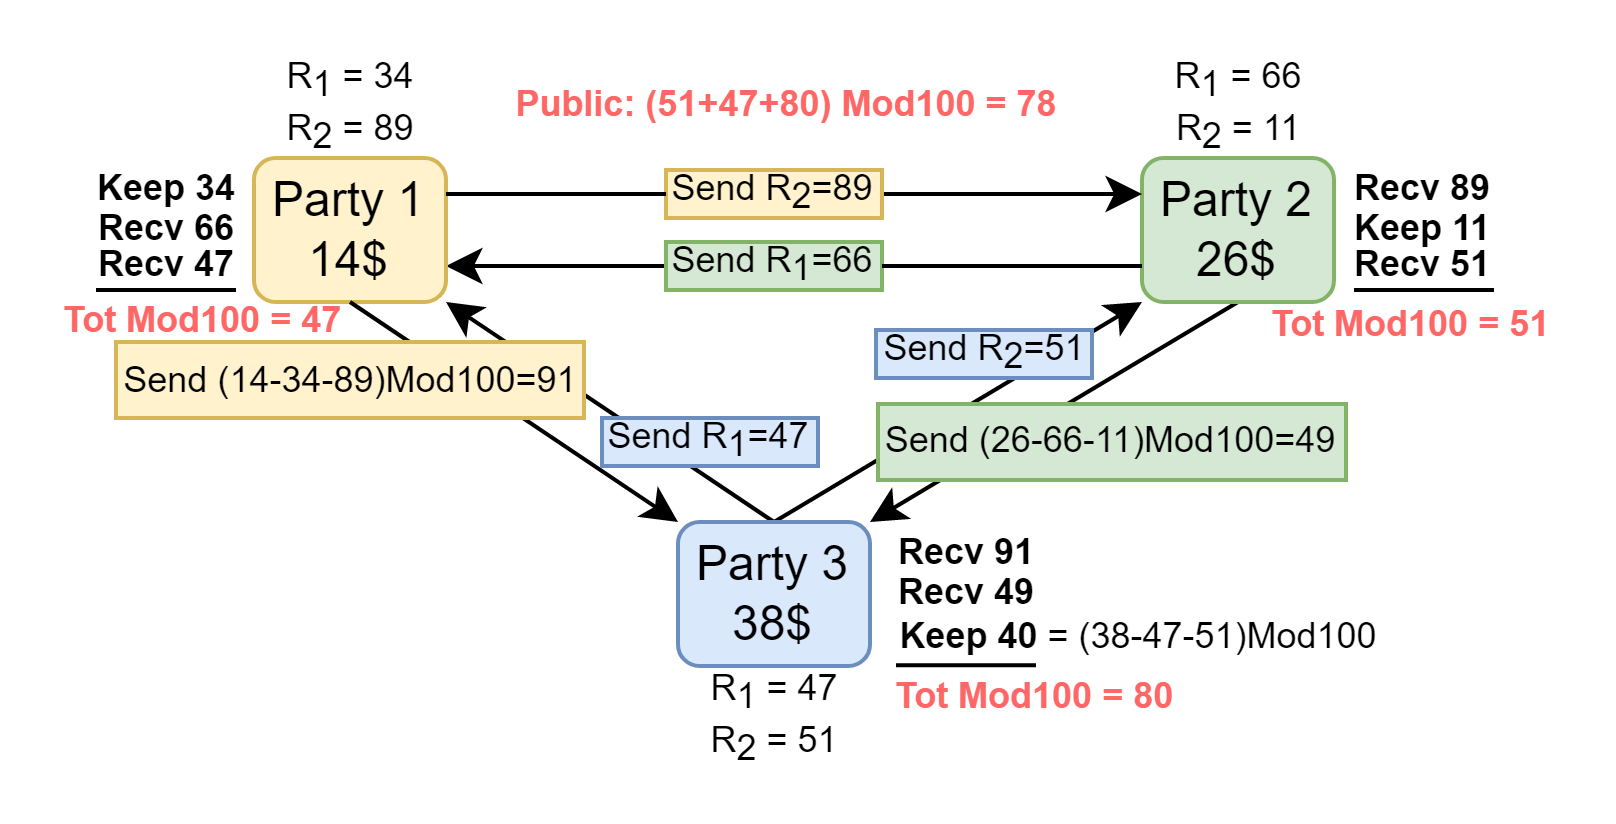
\includegraphics[width=0.7\textwidth]{image/secret_sharing/inputprivacy.png}
    \caption{(3,3) SMC Scheme}
    \label{fig:inputprivacy}
\end{figure}
\end{example}
\section{Verifiable Secret Sharing}
Supponiamo uno scenario in cui viene fatta una donazione di 10\$, ma viene comunicato che l'importo donato è di 1000\$. Lo schema di Shamir (\cref{thm:tnsecret}) è vulnerabile sul lato autenticazione, perché un input peer/ trusted party potrebbe \textit{"barare"} o, più semplicemente, non ha un modo per verificare che il segreto inserito è corretto.\\
Un modello di attacco che sorge in questo frangente, è il seguente:
\begin{definition}[Honest-but-Curious Model]\label{def:honestcurious}
Modello di attacco nel quale si vuole scoprire il segreto di un sistema, seguendo le regole del sistema stesso.
\end{definition}
Abbiamo bisogno di un modo di controllare che le regole del protocollo vengano seguite per intercettare e bloccare eventuali cheater.\\
\begin{remark}
Sia Dealer che Player possono essere cheater. I primi comunicando segreti inconsistenti, i secondi comunicando risultati che possono essere usati per manipolare la ricostruzione finale.
\end{remark}
Riassumendo, abbiamo bisogno di due proprietà:
\begin{itemize}
    \item \textbf{Malicious Dealer:} Una qualsiasi parte deve verificare che lo \textbf{share condiviso} sia consistente.
    \item \textbf{Cheating Parties:} Le parti devono verificare se uno \textbf{share rivelato} è consistente.
\end{itemize}
L'idea alla base dei protocolli aggiuntivi che vedremo è quella di creare un binding tra il segreto e ciò che viene rivelato. Questo binding è detto \textbf{Crypto Commitment}
\begin{theorem}[Feldman Verifiable Secret Sharing]\label{thm:feldvss}
Come Dealer:
\begin{enumerate}
    \item Genera polinomio random $p(x)$ di grado $t-1$ tale che $p(0)=s$.
    \item Distribuisci uno share per ogniuna delle $n$ parti: $(x_i, y_i)$, con $y_i=p(x_i)$. Tipicamente $x_i=i$.
    \item \textbf{Per ogni coefficiente} del polinomio, \textbf{compreso il segreto}, comunicare \textbf{pubblicamente}:
    \[c_0=g^s;\,c_1=g^{a_1};\,\dots,\,c_{t-1}=g^{a_{t-1}}\]
    Calcolati con \textbf{algebra modulare}\footnotemark rispetto un \textbf{numero primo}.
\end{enumerate}
\footnotetext{\textsuperscript{\thefootnote}Il calcolo modulare introduce il problema del discrete log, che rende difficile il calcolo dell'esponente.}
Come Verifier:
\begin{enumerate}
    \item Ogni parte riceve il suo share $(x_i, y_i)$, con $y_i=p(x_i)$.
    \item \textbf{Check Malicious Dealer:} Verifico che lo share ricevuto sia valido calcolando in $\bmod{P}$
    \begin{equation*}
        \begin{aligned}
            &c_0\cdot c_1^{x_i}\cdot c_2^{x_i^2}\cdot ...\cdot c_{t-1}^{x_i^{t-1}}=
            g^s\cdot\prod_ {k=1}^{t-1}g^{a_k x_i^k}=\\
            &=g^{s+a_1x_i+a_2x_i^2+\dots+a_{t-1}x_i^{t-1}}=g^{p(x_i)}
        \end{aligned}
    \end{equation*}
    \item Controlla che il risultato ottenuto sia uguale a $g^{y_i}$, con $y_i$ lo share della parte.
\end{enumerate}
\end{theorem}\pagebreak
\begin{note}
Stiamo usando la proprietà di omomorfismo dello schema di shamir, per verificare che mon ci sono state alterazioni negli share inviati.
\end{note}
\begin{definition}[Feldman Commitment]\label{def:commitment}
L'\textbf{"impegno"} nello schema di Feldman è il coefficiente $c=g^x\bmod{P}$, che impedisce a chi riceve il segreto di conoscere il valore di $x$.\\
Al fine di essere robusto un commitment di Feldman deve soddisfare:
\begin{itemize}
    \item \textbf{(Computational) Hiding:} il ricevente \textbf{non} dovrebbe poter dedurre niente sul segreto inviato.
    \item \textbf{(Perfectly) Binding:} Chi invia il commitment non può trovare un altro $x'$ tale che $g^{x'}=c$.\footnotemark
\end{itemize}
\footnotetext{\textsuperscript{\thefootnote}E' fondamentale ricordare che $x$ non può essere scelto in modo qualunque, altrimenti è facile trovare una collisione, vedi \cref{eq:eulertot}.}
\end{definition}
\begin{note}
Se il commitment fosse stato fatto con una funzione Hash, avremmo avuto la proprietà della computational hiding e perfectly binding se avessimo usato una funzione hash forte. Il problema è che siamo limitati a segreti di dimensione elevata per garantire sufficiente protezione, che comunque potrebbe non essere sufficiente nel tempo.
\end{note}
Vedremo successivamente dettagli aggiuntivi \textbf{necessari} affinché lo schema di Feldman possa funzionare. Per il momento, è importante capire che i valori di \textbf{g,p} \textbf{devono essere scelti in modo appropriato}:\\
\begin{remark}
Per come è definito il commitment di Feldman, $c_0=g^s$ lascia trapelare informazioni sul segreto. Se $s$ è piccolo, un dictionary attack può trovare il suo valore:
\begin{algorithmic}[1]
\For {$x$ in $[1,1000]$}
\If {$g^x == c_0$}
\State Secret Found
\EndIf
\EndFor
\end{algorithmic}
\end{remark}
\begin{note}
E' dimostrato che \textbf{è impossibile} costruire dei commitment che siano contemporameamente perfectly hiding e perfectly binding. Tuttavia, è possibile costruire commitment che siano perfectly hiding \textbf{al costo} di essere computational binding.
\end{note}\pagebreak
\subsection{Pedersen Commitment}
La costruzione di Pedersen nasce per migliorare quella di Feldman, la cui proprietà principale era che il commitment era homomorfico, infatti 
\[Commit(a+b)=Commit(a)\cdot Commit(b)\rightarrow g^{a+b}=g^a\cdot g^b\bmod p\]
\begin{theorem}[Pedersen Commitment]\label{thm:pedersen}
Dati g,h pubblici, il commitment è definito come:
\begin{equation}\label{eq:pedersen}
    Commit(a,r)=g^a\cdot h^r\bmod P
\end{equation}
E gode della proprietà di homomorfismo:
\[    Commit(a+b,r_a+r_b)=g^{a+b}\cdot h^{r_a+r_b}\bmod P=g^{a}h^{r_a}\cdot g^{b}h^{r_b}=Commit(a,r_a)\cdot Commit(b,r_b)
\]
Inoltre:
\begin{itemize}
    \item \textbf{Perfectly Hiding:} $c(a,r)=g^a\cdot h^r\bmod P$ può essere un commitment \textbf{per qualsiasi valore}. Formalmente: $\forall a'\ne a\,\exists !r':$ 
    \[commit(a',r')=g^{a'}\cdot h^{r'}\bmod P=g^a\cdot h^r\bmod P=commit(a,r)\]
    \item \textbf{Computationally Binding:} il Sender non dovrebbe essere in grado di trovare $a'$ ed un $r'$ associato, a meno di conoscre $log_g h$. 
\end{itemize}
\end{theorem}
\begin{proof}Proviamo che il Perdersen Commitment è Computationaly Binding:\\
Sia $h=g^w\rightarrow w=log_g h$. Supponiamo di conoscere $a,r$ e di scegliere $a'$. Vogliamo trovare un $r'$ associato ad $a'$ tale che
\begin{equation}\label{eq:proof}
    g^ah^r=g^{a'}h^{r'}
\end{equation}
Allora:
\begin{equation*}
    g^ag^{wr}=g^{a'}g^{wr'}\rightarrow     g^{a+wr}=g^{a'+wr'}
\end{equation*}
L'ultima equazione è vera se solo se: $a+wr=a'+wr'$. Pertanto possiamo trovare $r'$ tale che:
\[r'=w^{-1}(a-a'+wr)\]
Ricordando che le operazioni sono fatte in modulo, dato un $w$, possiamo calcolare qualsiasi collisione dei commitment, quindi non avremmo binding.\\
Per risolvere il problema, comunque, \textbf{devo poter invertire il discrete logarithm} e trovare $w$.
\end{proof}\pagebreak
\begin{definition}[Pedersen VSS]\label{def:pedvss}
Come Dealer:
\begin{enumerate}
    \item Genera due polinomi, shamir-like, tali che:
    \begin{equation*}
        \begin{aligned}
            f(x)&=s+a_1x+a_2x^2+...+a_{t-1}x^{t-1}\\
            f'(x)&=r+b_1x+b_2x^2+...+b_{t-1}x^{t-1}
        \end{aligned}
    \end{equation*}
    Dove $s,r$ sono i segreti da non rivelare, $a_i,b_i$ sono i coefficienti random.
    \item Invia alla parte i-esima un doppio share: $(x_i,y_i,z_i)$ con $y_i=f(x_i),z_i=f'(x_i)$.
    \item Pubblica commitment secondo Pedersen: $c_0=g^sh^r,c_1=g^{a_1}h^{b_1},...,c_{t-1}=g^{a_{t-1}}g^{b_{t-1}}$.
\end{enumerate}
Come un Verifier:
\begin{enumerate}
    \item La parte i-esima riceve lo share $(x_i,y_i,z_i)$ con $y_i=f(x_i),z_i=f'(x_i)$.
    \item Verifico ($\bmod P$) come in Feldman (\cref{thm:feldvss}), ma verifico la quantità $g^{y_i}h^{z_i}$.
\end{enumerate}
\end{definition}
\begin{note}
Applicando questo schema ad un esempio, senza prendere degli accorgimenti, non produrrebbe un risultato corretto. Dimostrazione tramite foglio di calcolo mathematica.
\end{note}
\subsection{Prime for Dummies}
Introduciamo la definzione di Gruppo:
\begin{definition}[Group]\label{def:group}
Un gruppo \textbf{(G,$\circ$)} è un insieme  nel quale viene definita un operazione, indicata con $\circ$.\\
Per un gruppo valgono le seguenti proprietà:
\begin{itemize}
    \item \textbf{Chiusura:} $\forall g_1,g_2\in{G}$ $g_x=g_1\circ g_2$.
    \item \textbf{Identità:} $\exists I\in{G}:\,g\circ I=I\circ g=g$.
    \item \textbf{Inversa:} $\forall g\in G, \exists g^{-1}\in G:\,g\circ g^{-1}=I$.
    \item \textbf{Associativa:} $\forall g_1,g_2,g_3 \in G$ vale che: $(g_1\circ g_2)\circ g_3=g_1\circ (g_2\circ g_3)$
\end{itemize}
\end{definition}
\begin{corollary}[Abelian Group]\label{cor:abelian}
Se per un gruppo (\cref{def:group}) \textbf{vale la proprietà di commutatività}, allora è detto \textbf{Abeliano}.
\end{corollary}
Il gruppo usato nelle moltiplicazioni della costruzione di Pedersen è il gruppo \textbf{Zp\textsuperscript{*}}.
\begin{definition}[Zp\textsuperscript{*}]
Gruppo basato sulla moltiplicazione di numeri interi in modulo P, dove P è un numero primo.
\begin{remark}
Per costruzione presenta un numero finito di $P-1$ elementi da $1$ a $p-1$, vedi \cref{eq:eulertot}. 0 è escluso.
\end{remark}
\end{definition}
\begin{note}
Se avessimo avuto la commutatività, avremmo avuto un campo: $\mathcal{F}p$
\end{note}\pagebreak
\begin{remark}
Tre proprietà su quattro sono ovviamente soddisfatte, compresa la commutatività. Per quanto riguarda l'inversa però abbiamo il problema che in modulo non esiste sempre l'inversa, a meno che questo non sia fatto secondo un numero primo, per questo è necessario.\footnote{Per calcolare l'inversa si può usare l'Algoritmo di Euclide Esteso (\cref{def:exteuc})}
\end{remark}
Per un gruppo basato sulla moltiplicazione, un esponente equivale al prodotto di $k$ volte della stessa base. 
\begin{definition}[Generator of Group of Order m]
Per un gruppo esiste sempre un elemento $g$ tale che ${g^0,g^1,\dots,g^{m-1}}$ è un insieme di $m$ elementi appartenenti a $G$.\\
\begin{property}[Prime-Order Group]
Un gruppo è di ordine primo se $m$ è un numero primo. Questo implica che ogni suo elemento, a parte l'identità, è un generatore.
\end{property}
\begin{remark}
Un gruppo $\mathcal{Z}_p^*$ ha ordine $p-1$, che è pari e non primo.
\end{remark}
\end{definition}
\begin{example}[ $Z_{11}^*$]
Consideriamo un insieme di elementi da 1 a 10: $G=\{1,2,3,4,5,6,7,8,9,10\}$ per il gruppo $Z_{11}^*$. Chi sono i generatori di questo gruppo?
\begin{itemize}
    \item \textbf{g=2:} $\{2,4,8,5,10,9,7,3,6,1\}$. E' un generatore.
    \item \textbf{g=3:} $\{3,9,5,4,1,3,9,5,4,1\}$. \textbf{Non} è un generatore. C'è un sottogruppo di ordine 5.
    \[\dots \text{3,4,5,9 non sono generatori, 6,7,8 si}\dots\]
    \item \textbf{g=10:} $\{10,1,10,1,10,1,10,1,10,1\}$. \textbf{Non} è un generatore, sottogruppo di ordine 2.
\end{itemize}
\begin{note}
La dimensione dell'insieme è data dal prodotto della dimensione dei due sottogruppi: $10=2\cdot5$. Si potrebbe dimostrare, ma non lo facciamo.
\end{note}
\label{exam:grouporder}
\end{example}
\begin{theorem}[Group Order]
L'ordine di un gruppo è dato dalla fattorizzazione della dimensione del gruppo.
\end{theorem}
Quello che abbiamo descritto implica che gli stessi numeri primi che usiamo in crittografia devono soddisfare una proprietà che chiamiamo:
\begin{definition}[Strong Primes]
Un numero primo $p$ è detto \textbf{Strong} se:
\begin{equation}\label{eq:strongp}
    p=2q+1,\,q\text{ è un numero primo}
\end{equation}
\end{definition}
Quindi, il gruppo $Z_p^*$ che ha ordine $p-1$, in realtà ha ordine $2q$. Quindi, \textbf{qualsiasi} membro $x$ del gruppo (\textbf{tranne} 1 e $p-1$) può fare una delle due cose:
\begin{itemize}
    \item Genera l'intero gruppo.
    \item Genera un sottogruppo di ordine primo $q$.
\end{itemize}
\begin{note}
Ogni volta che vogliamo un numero primo \textbf{grande}, vogliamo che sia $p$ che $q$ siano grandi. Altrimenti $p-1$ può essere fattorizzato in numeri più piccoli. 
\end{note}
\begin{remark}
C'è una proprietà molto importante che possiamo dedurre dall'esempio \ref{exam:grouporder}: si può vedere che i numeri che sono generatori del gruppo sono in realtà tutti quei numeri che non possono essere espressi come radici quadrate.
\end{remark}
\begin{definition}[Quadratic Residue]\label{def:quadres}
Un numero $x\in Z_P^*$ è un residuo quadratico se ammette radice quadratica nel gruppo. Ovvero:\[\exists a:\,a^2\bmod{p}=x\]
\end{definition}
\begin{definition}[Quadratic Residue Subgroup $QR$]\label{def:qr}
E' un sottogruppo formato da tutti gli elementi $x\in Z_p^*$ che sono residui quadratici.
\end{definition}
\begin{example}
Per $Z_{11}^*$ il $QR=\{1,3,4,5,9\}$
\end{example}
Vale il seguente teorema:
\begin{theorem}[Subgroup Generator]
Se $x$ è un residuo quadratico, allora genera un sottogruppo di ordine $q=\frac{p-1}{2}$.\\
Inoltre, si può provare che:
\[a\in{QR}\Longleftrightarrow a^{\frac{p-1}{2}}=1\]
Questa operazione è detta \textbf{Legender Symbol}
\end{theorem}
\begin{corollary}
Se $p$ è un numero \textbf{primo forte}, allora, $QR_p$ ha \textbf{prime-order} $q$.
\end{corollary}
\begin{note}
Questo significa che in uno schema di Pedersen se $g\in {QR_p}$ allora quando calcoliamo l'esponenziale lo stiamo facendo in modulo $q$.
\end{note}
%TODO: nserire esempio vss corretto
\pagebreak
\section{Distributed Secret Sharing}
\begin{problem}E' possibile generare una coppia \textbf{\{$\text{Pub}_k$,$\text{Priv}_k$\}} tale che tutti conoscano la chiave pubblica e nessuno quella privata?
\end{problem}
Questo scenario è coperto dai sistemi crittografici \textbf{\textit{DLog-based}}, dove la private-key $x$ è nascosta dalla public key $g^x$. Schemi del genere sono utili quando la chiave privata deve essere rivelata in un secondo momento (ad esempio in caso in cui si deve cifrare un messaggio che nessuno può aprire a meno di speciali condizioni), o non deve \textbf{mai} essere rivelata ma le sue caratteristiche sono necessarie.\\
Lo schema di condivisione funziona nel seguente modo:
\begin{definition}[Distributed Ssecret Sharing]\label{def:dss}
Consideriamo uno schema di secret sharing distribuito con $x$ chiave privata e $g^x$ chiave pubblica. Procediamo nel seguente modo:
\begin{enumerate}
    \item Ogni parte genera indipendentemente un segreto $a_{0,i}$
    \item Ogni parte genera indipendentemente il suo polinomio di grado $t-1$ con termine noto $a_{0,i}$.
    \item Ogni parte invia uno share $p_i(k)$ alle altre parti, e trattiene $p_i(i)$.
    \item Ogni parte calcola la somma degli share e \textbf{la trattiene per se}. Questa somma sarà la somma dei segreti, che fino ad ora sono rimasti privati.\\
    \begin{remark}
    Se ogni parte comunicasse il proprio risultato $y_i$ sarebbe possibile per interpolazione calcolare $S=\sum_i a_{0,i}$
    \end{remark}
    \item Invio in broadcast un commitment per $a_{0,i}$: $g^{a_{0,i}}$. Moltiplicando i quattro commitment possiamo calcolare $g^s$.
\end{enumerate}
\end{definition}
\begin{figure}[h]
\vspace{-10pt}
    \centering
    \begin{subfigure}[b]{0.5\textwidth}
    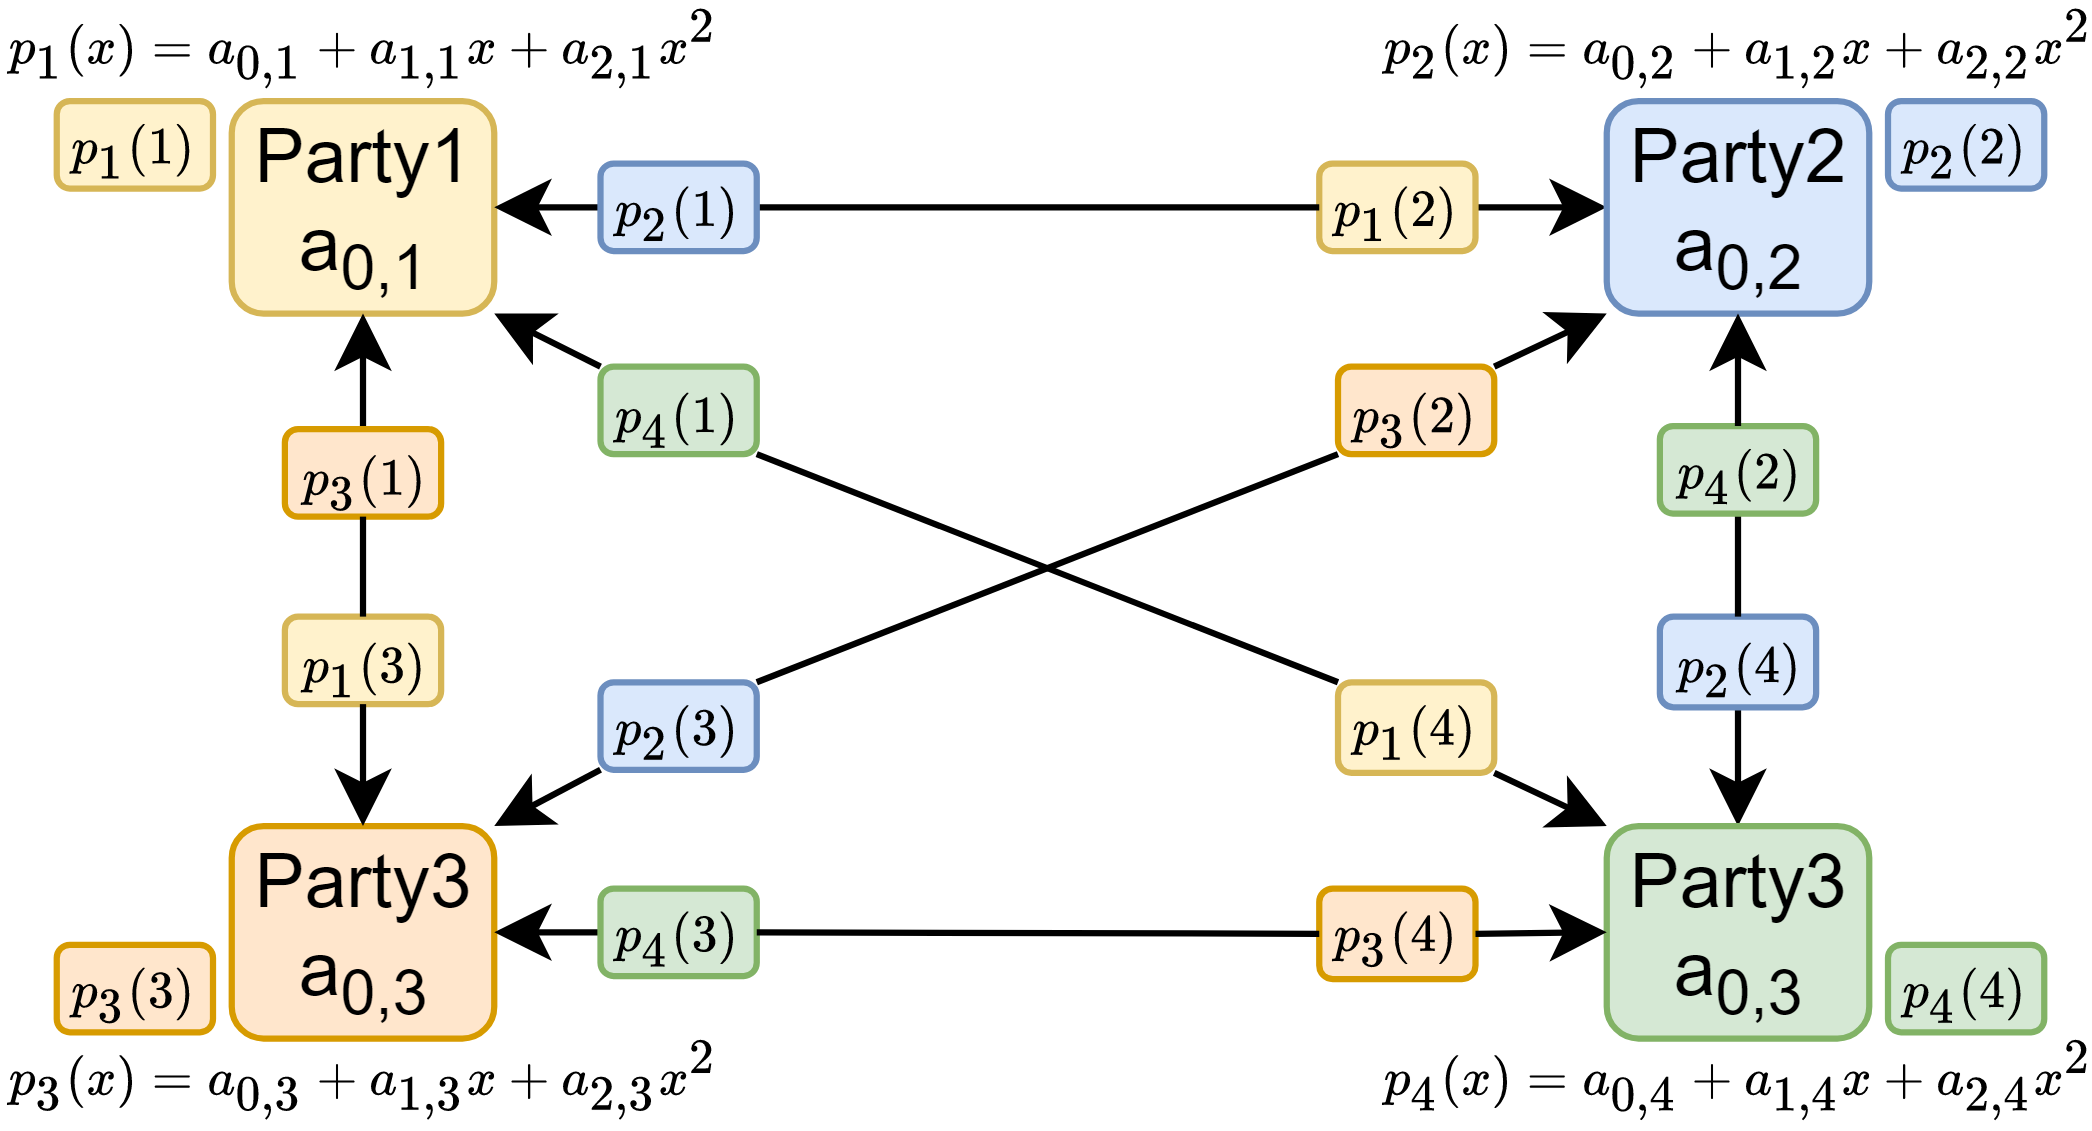
\includegraphics[width=\textwidth]{image/secret_sharing/dssa.png}
    \caption{Sharing phase}
    \label{fig:dssa}
    \end{subfigure}\quad
    \begin{subfigure}[b]{0.48\textwidth}
    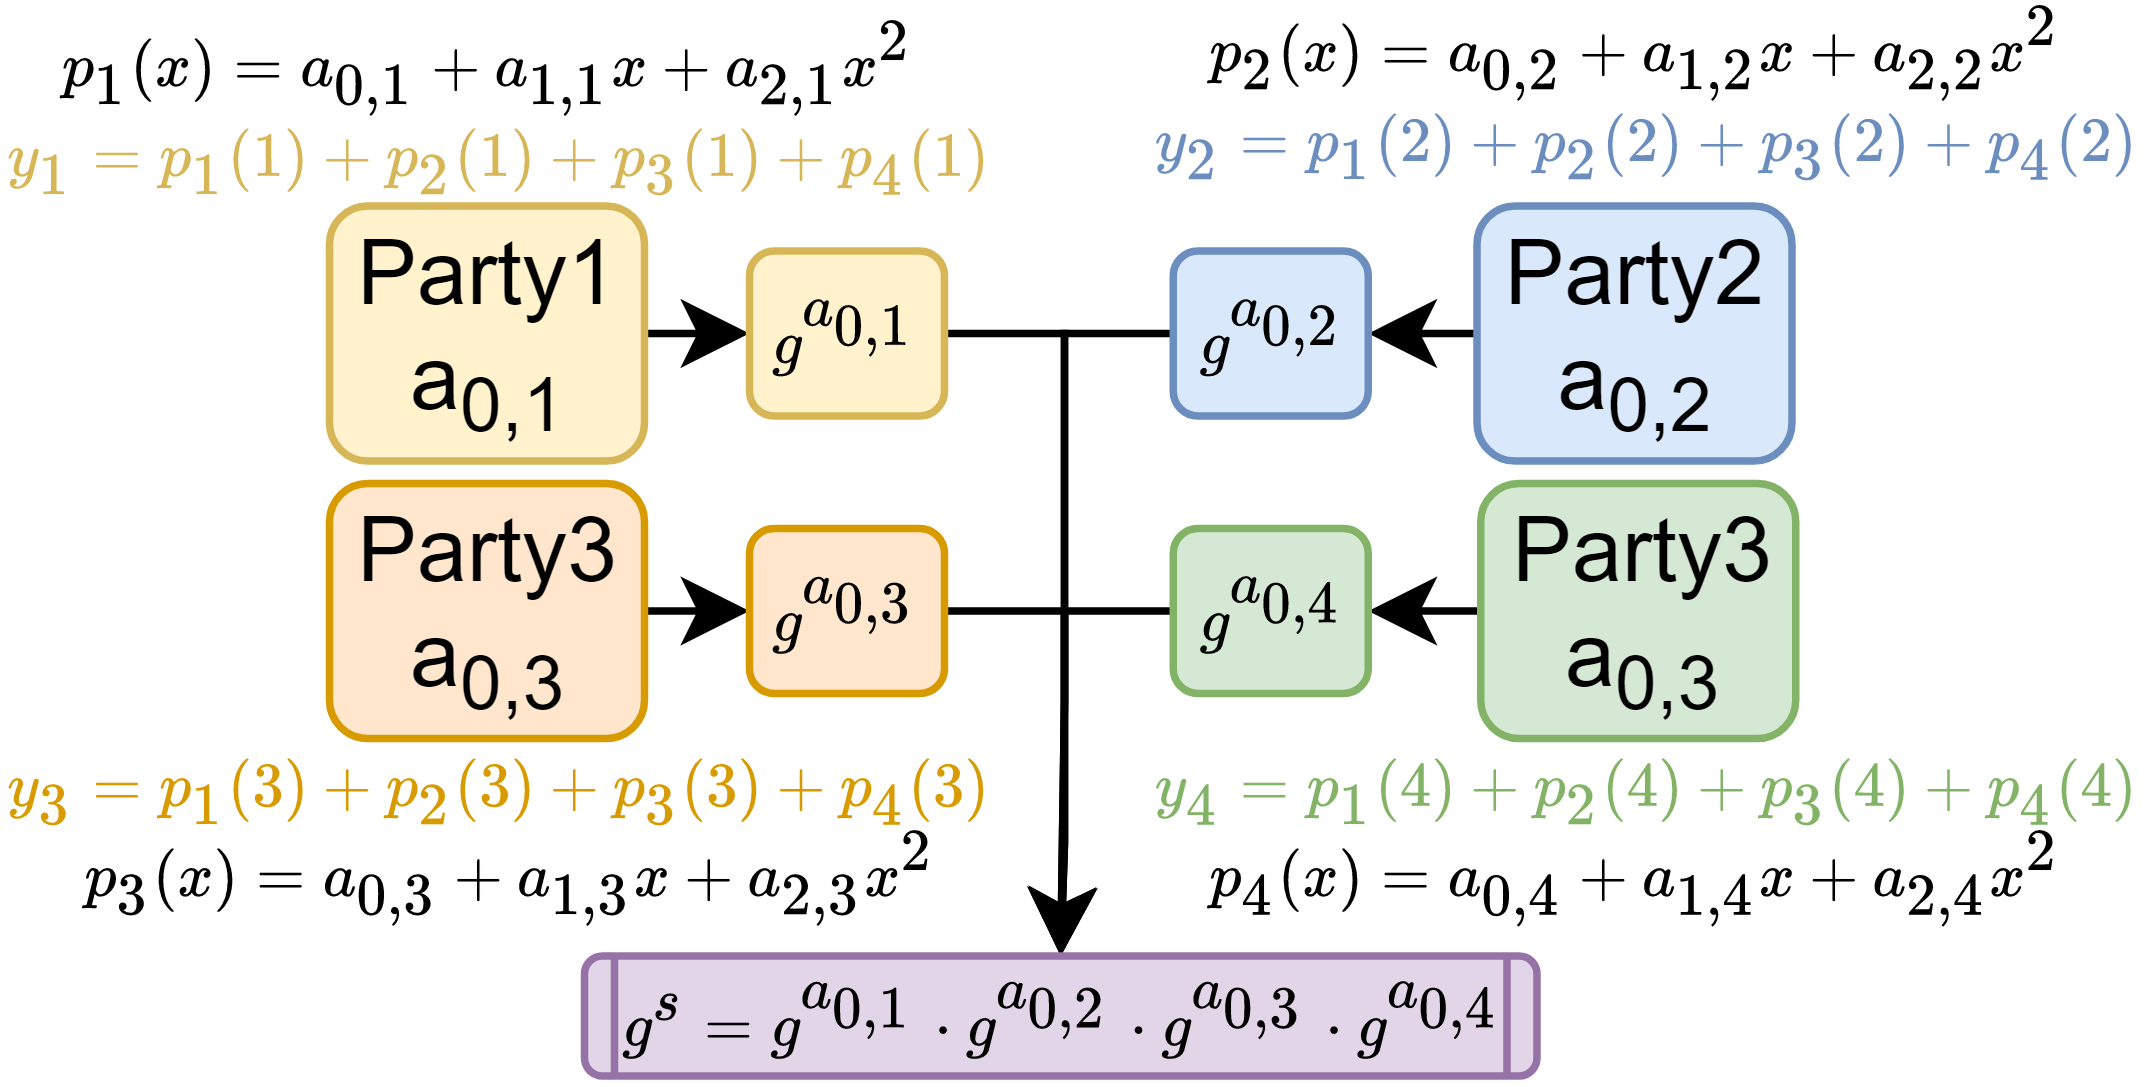
\includegraphics[width=\textwidth]{image/secret_sharing/dssb.png}
    \caption{$g^s$ computation}
    \label{fig:dssb}
    \end{subfigure}
    \caption{DSS Example with (3,4) scheme}
\end{figure}
